%!TEX root =/Users/andreasmller/Documents/DTU/Computerspil/scienceman/report/report.tex
\section{Implementation} % (fold)
Incorporation and tweaking of the chipmunk physics engine in a way that provides a solid gameplay takes a huge amount of work, and creating a simulation based game involves an endless amount of unforeseen complications. We have therefore reduced the game prototype to a single level, which focuses on the combat involving physical objects. Our prototype does not include a heads up display, or any type of cut scenes to drive the story forward (it technically does not even include a story). These elements may be complex to design properly, but they are trivial to implement. We have therefore chosen to focus on implementing the physics powers described in section 2. This is where the game differs from all other existing platform games, and this is where the challenges of the implementation lies.
\subsection{Project Structure}

The project structure is based that of the Mr. Fuze game, and some of the features are copied directly from this game.These features include loading levels from image files, and the Camera class, which centers the viewport around the player. The level loading feature makes it very easy to create new levels, and makes any basic image editor into a level editor. This gave us a good IDEA / ALTER structure to work from.

\subsection{Graphics}
The game graphics are very crude and simple, since none of the developers have any creative skills what so ever. We have copied the background and platform textures from a python game name robot toast. The characters are simple stickfigures, which adequately serves as avatars, but are not exactly pleasing to the eye. The crown of the sprite collection is the crates, which comes in two different sizes and colors, and has an unseen level of detail compared to the stickfigures.

\subsection{Physics}

The physics implementation is based on pumunk. All our world objects, which inherits from sprite, also contain a body and shape. Pymunk simulates their movement, and sprites are then moved to the body position, and turned based on the angle. Objects are never directly moved by the program, only by applied forces and impulses.

\subsubsection{Game world}

All non-moving platform, are static polygons with infinite mass and inertia, preventing them from being moved while being part of the physics world. 

\subsubsection{Player movement}

The player is a simple rectangle polygon in the physics world. He has a fairly large mass and infinite inertia. This allows him to be hit by the crates he throws around, and be pushed around by them to some extend. Infinite inertia makes sure he's never knocked over or flipped. Movement is done by applying impulse to his body, but with a limit to his maximum speed. This gives acceleration to his movement, while still having him affected by the momentum of objects he collides with. Jumping is similarly done by applying a lateral impulse, he cannot jump again until he collides with another physics object, to allow him to jump from the top of crates. This is one of the places where a compromise have had to be made, and the implementation doesn't quite feel right yet. At the time of writing any collision anywhere on the player, is adequate to a allow jumping again, which mean a player with a crate on his head, can jump straight up forever. Several solutions present them selfs, our preferred being only allowing a jump after a collision with feet of the player, having a upward normal vector. This solution opens up for a rather interesting move, where the player jumps while above a crate, then force pulls it up to his feet. This could in theory be repeated forever, unless power limitations prevent it. This move can be mimicked under current circumstances, and is a rather difficult move, making it more of a feature than a bug if implemented in such a way. Currently stopping feels somewhat odd, since the player with his high momentum, takes a while to stop on his own with using only friction with the surface.

\subsubsection{Player abilities}

\textbf{Force push / pull}

Force push as expected pushes all objects not nailed down, within and area away from the player, and the force pull vice verca.

\begin{figure}[h]
\begin{center}
 	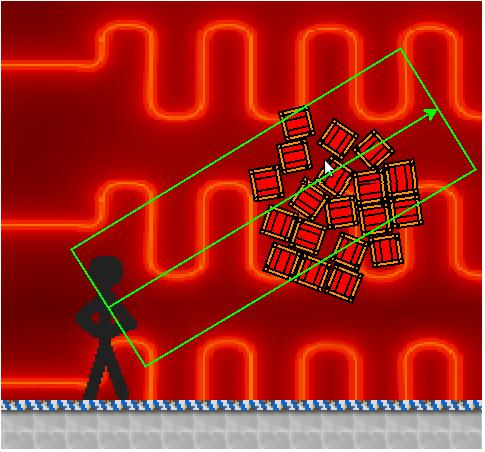
\includegraphics[width=8cm]{pics/push}
	\caption{Force power area of effect}
	\label{fig:force}
\end{center}
\end{figure}

 The power eminates from the player, and is directed towards the current cursor position. These force power have fixed ranges, and all non-static physics objects within the area is applied with a fixed impulse, making smaller object more affected than larger. Both moves can be used aggresively pushing boxes in front of enemies, or pulling crates behind him. But also more creative maneuvers, like pulling crates towards yourself, jumping over them, letting them hit enemies on the other side of the player. 
\\ \\
\textbf{Gravity well}

This power pull all nearby objects towards the cursor. The cursor can be moved, while "holding" object, and can be used in a number of creative ways. The power proved somewhat difficult to implement, and is based on some slightly selfinvented math. The original implementation was to apply a force on all objects within range, which had several problems. All object built quite a large momentum towards the cursor, making them fly almost as far away as they had originally been on the other side of the cursor. Secondly all the objects oscillated horizontally around the cursor.

\begin{figure}[h]
  \begin{center}
 	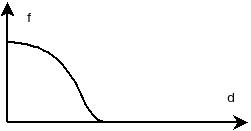
\includegraphics[width=6cm]{pics/force}
	\caption{Force of gravity well based on distance}
	\label{fig:Gravity}
\end{center}
\end{figure}

The final version is have a polyminally growing force towards the cursor, with a cap on the maxiumum force. It also have a velocity dampening of 1\% to avoid oscilation which works quite well.
\\ \\
\textbf{Timestop / Timeslow}

Not all of the abilities planned in the original design document have been implemented. A timestop or timeslow ability was dropped, which originally was planned to be used to enable more complex maneuvers with the physics powers. Things like jumping on crates falling in mid air and dodging enemy bullets. This ability was party dropped due to time constraints, but the game currently doesn't feel like it needs this ability. The higher pace and reaction time give an extra sence of danger, and makes difficult moves feel more rewarding when they succeed. It could have been implemented by reducing the simulating step count, while retaining the pygame tick framerate.

